\documentclass[dvipdfmx]{beamer}

\usepackage{graphics}
\usepackage{amsmath}
\usepackage{amssymb}
\usepackage{ascmac}
\usepackage{txfonts}
\usepackage{bm}
\usepackage{docmute}
\usepackage{tikz}
\usetikzlibrary{calc}
\usetikzlibrary{intersections}

\usetheme{Madrid}
\usefonttheme{professionalfonts}


\title{5月第1課題}
\author{近藤 綜太}

\begin{document}
	\maketitle
	\begin{frame}{はじめに}
		緊急事態宣言が延長され,休校期間が伸びそうになってきました.
		そこで,学校がなくとも学習の進度を守れるようにここで
		いくつかの課題を出していきたいと思います.

		発展的な問題を出すこともあるので,
		グループのみんなで相談しながら解いてください.
	\end{frame}

	\begin{frame}{問題1}
		図の四角形 $\mathrm{ABCD}$は平行四辺形である.
		この平行四辺形の面積を二等分する直線のうち,
		傾きが1であるものを求めよ.
		\begin{figure}[htbp]
			\centering
			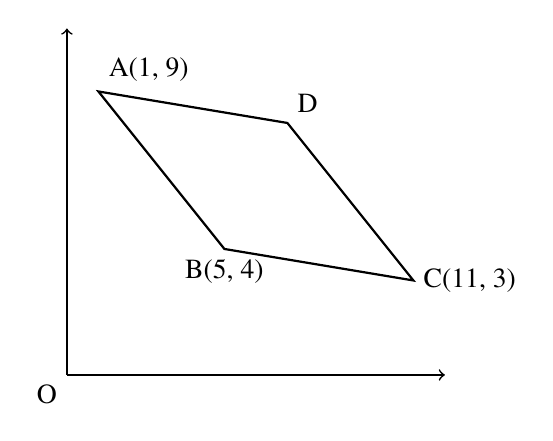
\begin{tikzpicture}[scale = 0.4]
				\draw[semithick, ->] (0, 0)node[below left]{O}--(12, 0);
				\draw[semithick, ->] (0, 0)--(0, 11);

				\coordinate[](a) at (1, 9);
				\coordinate[](b) at (5, 4);
				\coordinate[](c) at (11, 3);
				\coordinate[](d) at (7, 8);

				\draw[thick] (a)node[above right]{A(1, 9)}--(b)node[below]{B(5, 4)}--(c)node[right]{C(11, 3)}--(d)node[above right]{D}--cycle;
			\end{tikzpicture}
			\caption{平行四辺形}
		\end{figure}
	\end{frame}

	\begin{frame}{問題2}
		\begin{columns}
			\begin{column}{0.5\textwidth}\centering
				\begin{figure}[htbp]
					\centering
						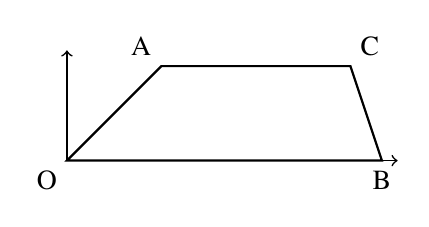
\begin{tikzpicture}[scale = 0.2]
							\draw[semithick, ->] (0, 0)node[below left]{O}--(21, 0);
							\draw[semithick, ->] (0, 0)--(0, 7);

							\coordinate[](a) at (6, 6);
							\coordinate[](b) at (20, 0);
							\coordinate[](c) at (18, 6);
							\draw[thick] (a)node[above left]{A}--(c)node[above right]{C}--(b)node[below]{B}--(0, 0)--cycle;
						\end{tikzpicture}
					\caption{台形}
				\end{figure}

				\begin{gather*}
					\mathrm{A}:(6, 6)\\
					\mathrm{B}:(20, 0)\\
					\mathrm{C}:(18, 6)
				\end{gather*}
			\end{column}

			\begin{column}{0.5\textwidth}
				以下の条件を満たす直線をそれぞれ求めよ.
				\begin{enumerate}
					\item 点Aを通り,台形AOBCの面積を二等分にする直線
					\item 点(12, 6)を通り,台形AOBCの面積を二等分にする直線
					\item 傾き1で,台形AOBCの面積を二等分にする直線
				\end{enumerate}
			\end{column}

		\end{columns}
	\end{frame}

	\begin{frame}{解答1-1}
		平行四辺形を二等分にする直線の引き方を考える.

		平行四辺形をその対角線で切ると,当然同じ形が1つでてくるので
		面積を二等分できる.ここから以下の図の2つの三角形の
		面積を考える.
		\begin{figure}[htbp]
			\centering
			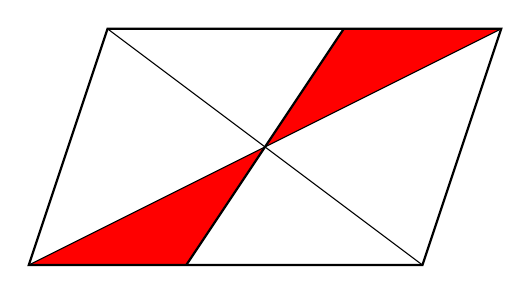
\begin{tikzpicture}[scale = 1.0]
				\coordinate[](a) at (0, 0);
				\coordinate[](b) at (5, 0);
				\coordinate[](c) at (6, 3);
				\coordinate[](d) at (1, 3);
				\coordinate[](m) at (3, 1.5);

				\fill[red] (a)--(m)--($(a)+(2, 0)$)--cycle;
				\fill[red] (c)--(m)--($(c)-(2, 0)$)--cycle;

				\draw[thick] (a)--(b)--(c)--(d)--cycle;
				\draw[thin] (a)--(c);
				\draw[thin] (b)--(d);

				\draw[thick] ($(a)+(2, 0)$)--($(c)-(2, 0)$);
			\end{tikzpicture}
			\caption{平行四辺形を二等分}
		\end{figure}
		対角線の交点を通るようにすれば赤い三角形の面積は等しくなる.

		このことを利用すれば,平行四辺形の2本の対角線の交点を
		通る直線が,平行四辺形を二等分するとわかる.
	\end{frame}

	\begin{frame}{解答1-2}
		平行四辺形の面積を二等分にする直線は2本の対角線の交点を通る直線
		であるとわかった.そして,2本の対角線の交点は
		それぞれの対角線の中点である.
		対角線ACの中点は(6, 6)なので,これを通る傾き1の
		直線が答えである.
		\[y=x\]
	\end{frame}

	\begin{frame}{解答2-1}
		面積を二等分するのだから,まずは全体の面積を計算する.

		\begin{align*}
			(\text{台形AOBC})&= \frac{1}{2}\times(\mathrm{AC}+\mathrm{OB})\times 6\\
							 &=96
		\end{align*}

		これの二等分だから分けた後の面積は48であるとわかる.
	\end{frame}

	\begin{frame}{解答2-2}
		点A を通り面積を二等分する直線を考える.
		点Aを通る直線が台形を分けるので次の場合が考えられる.
		\begin{enumerate}
			\item 線分BCと交わる
			\item 点Bを通る
			\item 線分OBと交わる.
		\end{enumerate}
		まずはこのどれに当てはまるのかを確認する必要がある.
		これは実際に点Bを通るときに面積がどのように分割される
		のかを確認すればいい.
		
		直線が点Bを通るとすると $\triangle\mathrm{ABO}$は
		\[\triangle\mathrm{ABO}= \frac{1}{2}\times20\times6=60>48\]
		となる.したがって,点Aを通り台形の面積を二等分する直線は
		線分OBと交わる直線であるとわかる.
	\end{frame}

	\begin{frame}{解答2-3}
		点Aを通り線分OBと交わる直線の線分OBとの交点をPとする.
		$\triangle\mathrm{APO}$の面積は
		\[\triangle\mathrm{APO}= \frac{1}{2}\times 6\times\mathrm{OP}\]
		これが48となる.
		\begin{gather*}
			\frac{1}{2}\times 6\times\mathrm{OP}=48\\
			\Leftrightarrow\mathrm{OP}=16\\
			\therefore\mathrm{P}\, (16, 0)
		\end{gather*}
		題意の直線は点A(6, 6),点P(16, 0)を通る直線なので
		以下の式である.
		\[y = - \frac{3}{5}x + \frac{48}{5}\]
	\end{frame}

	\begin{frame}{解答2-4}
		点(12, 6)を通る直線で台形を二等分することを考えると
		答えは困難を極める.まず点(12, 6)が何なのかを考える必要がある.

		この点はなんと,ちょうど上底の中点に位置している.
		ここから引いた直線で台形を二等分すると考えると簡単だ.
		上底の中点と下底の中点の両方を通る直線であれば,
		台形の面積を二等分できる.
		このことは各自確認してほしい.

		下底の中点は(10, 0)なので,求める直線は
		点(12, 6)と点(10, 0)を通る直線である.
		したがって答えは以下の式となる.
		\[y = 3x - 30\]
	\end{frame}


	\begin{frame}{解答2-5}
		最後の問題はかなりの高難度となっている.
		ここでは場合分けを使いながら,最後は方程式の計算によって
		答えを求める.

		まずは場合分けの話だ.台形が図の形であることから,
		傾き1の直線が台形を二つの部分に分けるのは次の場合が
		考えられる.
		\begin{enumerate}
			\item 線分ACと交わる
			\item 点Cを通る
			\item 線分BCと交わる
		\end{enumerate}
		ここでも1番目のときと同じように考える.
		点Cを通る場合を考える.そして,傾き1の
		直線と線分OBとの交点をQとする(Q(12, 0))と
		$\triangle\mathrm{CBQ}$の面積は
		以下で計算される.
		\begin{align*}
			\triangle\mathrm{CBQ} &= \frac{1}{2}\times \mathrm{BQ}\times 6\\
								  &= 24
		\end{align*}
		ここから求める直線は線分ACと交わることがわかる.
	\end{frame}

	\begin{frame}{解答2-6}
		\begin{columns}
			\begin{column}{0.5\textwidth}
				\begin{figure}[htbp]
					\centering
						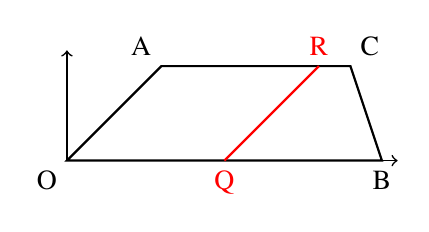
\begin{tikzpicture}[scale = 0.2]
							\draw[semithick, ->] (0, 0)node[below left]{O}--(21, 0);
							\draw[semithick, ->] (0, 0)--(0, 7);

							\coordinate[](a) at (6, 6);
							\coordinate[](b) at (20, 0);
							\coordinate[](c) at (18, 6);
							\draw[thick] (a)node[above left]{A}--(c)node[above right]{C}--(b)node[below]{B}--(0, 0)--cycle;
							\draw[thick, red] ($(c)-(2, 0)$)node[above]{R}--($(c)-(6, 6)-(2, 0)$)node[below]{Q};
						\end{tikzpicture}
					\caption{台形と直線}
				\end{figure}
				
			\end{column}

			\begin{column}{0.5\textwidth}
				台形に線分ACと交わる直線を引く.
				線分ACとの交点をR,線分OBとの交点をQとする.

				Rの座標を $(x, 6)$とすると,
				直線の傾きが1であることからQの座標は
				$x-6, 0$であるとわかる.

				ここから台形CBQRの面積を計算する.

			\end{column}
		\end{columns}
		
	\end{frame}

	\begin{frame}{解答2-7}
		まずは上底と下底を求める.
		\begin{align*}
			(\text{上底})&= 18 -x\\
			(\text{下底})&= 20 -(x-6) = 26-x
		\end{align*}
		ここから台形の面積の公式を使う.
		\begin{align*}
			(\text{台形CBQR}) &= \frac{1}{2}\times
			\{ (18-x)+(26-x) \}\times6\\
							  &= 3(44 -2x)
		\end{align*}
		これが48である $x$を求める.
		\begin{gather*}
			3(44-2x)=48\\
			\Leftrightarrow -2x = 16-44\\
			\therefore x = 14
		\end{gather*}
		したがって点C(14, 6)を通る傾き1の直線が答えとなり次式である.
		\[y =x -8\]
	\end{frame}

	\begin{frame}{解答2-8}
		(別解)

		四角形OARQが平行四辺形であることに気付いたら秒殺できる.
		\begin{gather*}
			(\text{四角形OARQ}) = \mathrm{OQ}\times 6=48\\
			\therefore\mathrm{OQ}=8
		\end{gather*}
		点(8, 0)を通る傾き1の直線は次の通り.
		\[y =x -8\]

		これでも十分な解答である.
	\end{frame}

\end{document}
>>>>>>> 43b99f2d66bf5ce86bfa866753e554c49a5d89f7:mathQuestion/question02.ltx
